\section{Appendix: Numerical Experiments}
\begin{frame}{Constant Velocity Case - Subsonic}
  \begin{figure}[H]
    \centering
    \begin{subfigure}{0.45\textwidth}
      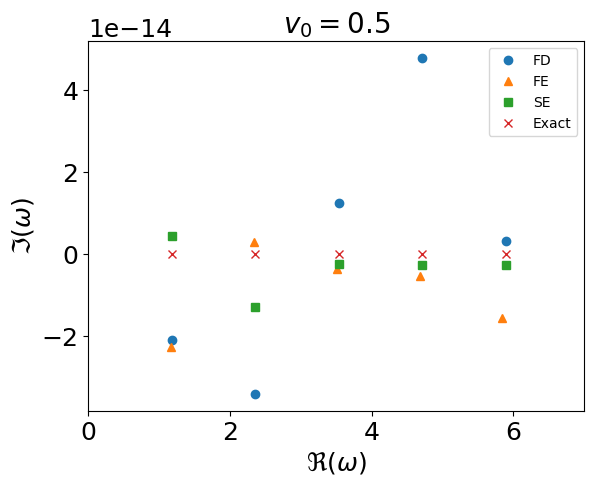
\includegraphics[width=0.9\linewidth]{figures/numerical-experiments/fixed-fixed/constant-v-v0=0.5}
      \caption{Dirichlet boundary, all modes are stable.}
    \end{subfigure}%
    \begin{subfigure}{0.45\textwidth}
      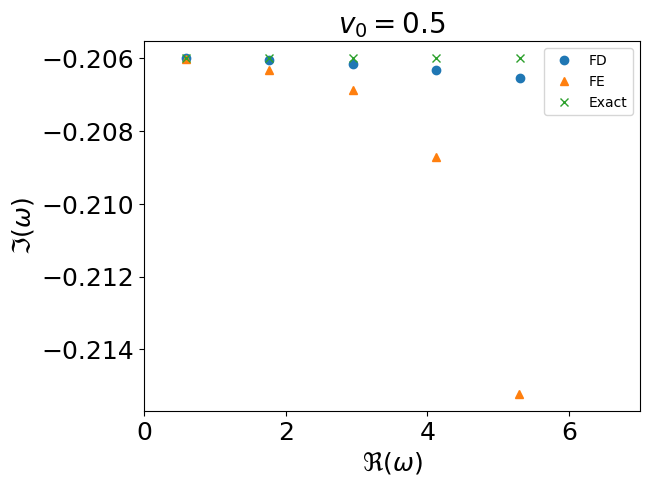
\includegraphics[width=\linewidth]{figures/numerical-experiments/fixed-open/constant-v-v0=0.5}
      \caption{Fixed-open boundary, all modes are stable.}
    \end{subfigure}
    \caption{Showing the first 5 eigenvalues. In the Dirichlet boundary case, all methods are close to the exact eigenvalues. Meanwhile, finite-difference method has higher accuracy than finite-element method in fixed-open case.}
  \end{figure}
\end{frame}


\begin{frame}{Constant Velocity Case - Supersonic}
  \begin{figure}[H]
    \begin{subfigure}{0.45\textwidth}
      \centering
      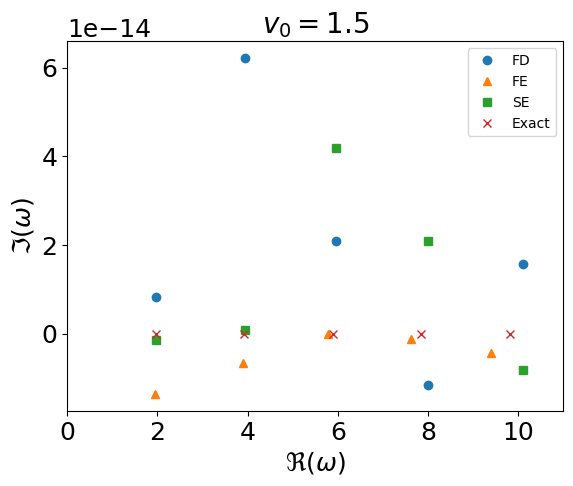
\includegraphics[width=0.9\linewidth]{figures/numerical-experiments/fixed-fixed/constant-v-v0=1.5}
      \caption{Dirichlet boundary, filtered modes are stable.}
    \end{subfigure}%
    \begin{subfigure}{0.45\textwidth}
      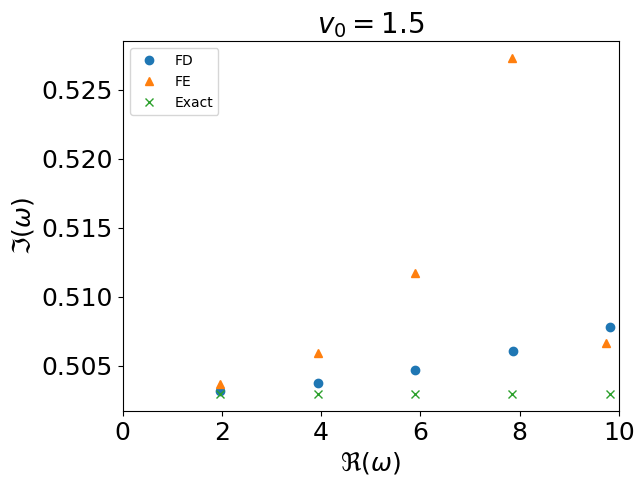
\includegraphics[width=\linewidth]{figures/numerical-experiments/fixed-open/constant-v-v0=1.5}
      \caption{Fixed-open boundary, all modes are unstable.}
    \end{subfigure}
    \caption{Showing the first 5 eigenvalues. In the Dirichlet boundary case, all methods are close to the exact eigenvalues. Meanwhile, finite-difference method has higher accuracy than finite-element method in fixed-open case.}
    \label{fig:constant-v-fixed-open}
  \end{figure}
\end{frame}

\begin{frame}{Subsonic Case}
  \begin{figure} [H]
    \centering
    \begin{subfigure}{0.45\textwidth}
      \centering
      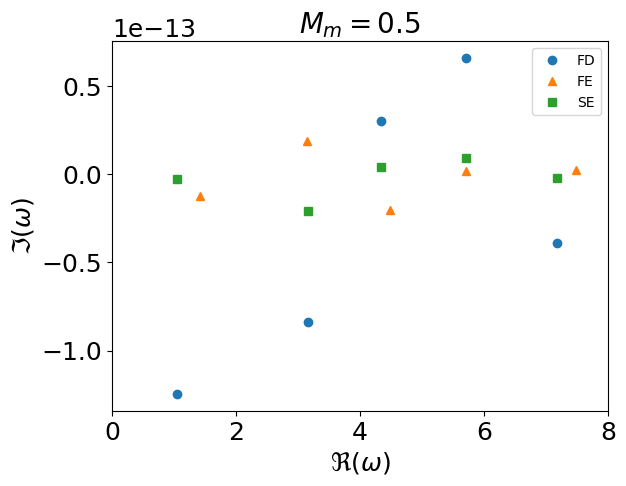
\includegraphics[width=\linewidth]{figures/numerical-experiments/fixed-fixed/subsonic-v}
      \caption{Dirichlet boundary, all modes are stable.}
    \end{subfigure}%
    \begin{subfigure}{0.45\textwidth}
      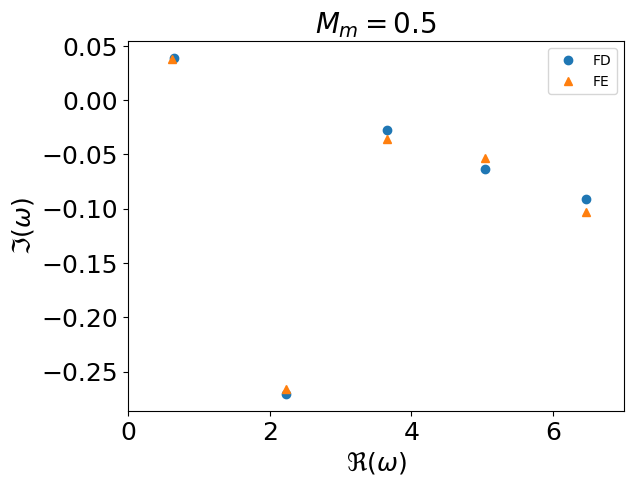
\includegraphics[width=\linewidth]{figures/numerical-experiments/fixed-open/subsonic-v}
      \caption{The ground mode is unstable, other modes are stable.}
    \end{subfigure}
    \caption{Showing the first 5 modes. It suggests that the subsonic flow in magnetic nozzle is stable.}
  \end{figure}
\end{frame}

\begin{frame}{Supersonic Case}
  \begin{figure} [H]
    \centering
    \begin{subfigure}{0.45\textwidth}
      \centering
      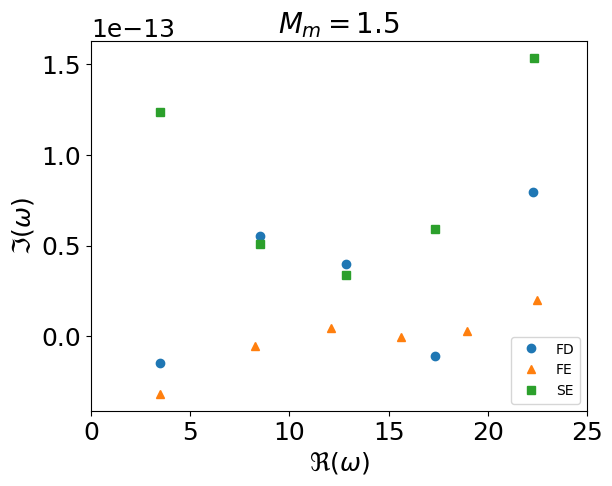
\includegraphics[width=\linewidth]{figures/numerical-experiments/fixed-fixed/supersonic-v}
      \caption{Dirichlet boundary, filtered modes are stable.}
    \end{subfigure}%
    \begin{subfigure}{0.45\textwidth}
      \centering
      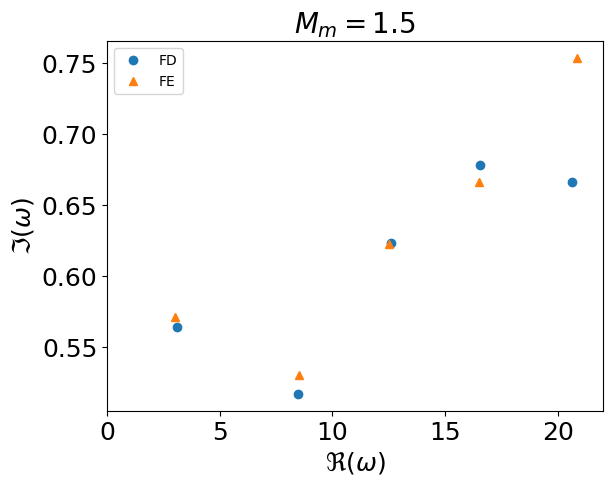
\includegraphics[width=\linewidth]{figures/numerical-experiments/fixed-open/supersonic-v}
      \caption{Fixed-open boundary, all modes are unstable.}
    \end{subfigure}
    \caption{This suggests that the supersonic flow is stable if the boundary is Dirichlet and unstable if the boundary is left-fixed-right-open.}
  \end{figure}
\end{frame}

\begin{frame}{Accelerating Case}
  \begin{figure} [H]
    \centering
    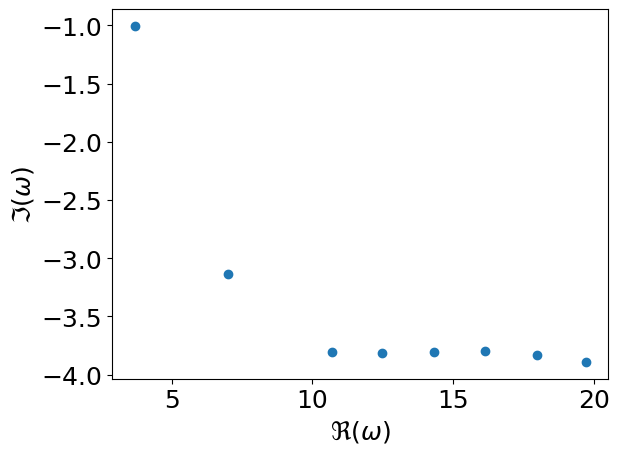
\includegraphics[width=0.7\linewidth]{figures/numerical-experiments/accelerating-v}
    \caption{All modes are stable.}
  \end{figure}
\end{frame}
